\documentclass{article}
\usepackage{amsmath}
\usepackage{graphicx}
\usepackage{float}
\begin{document}

%latex, bibtex, pdflatex x2 from terminal
\begin{center}
\textbf{\huge{Ph 20 Assignment 1}} \\
\textbf{\Large{David Shlivko}} \\
\textbf{\large{6 October 2017}}
\end{center}

\section{Lissajous Figures}

\begin{figure}[H]
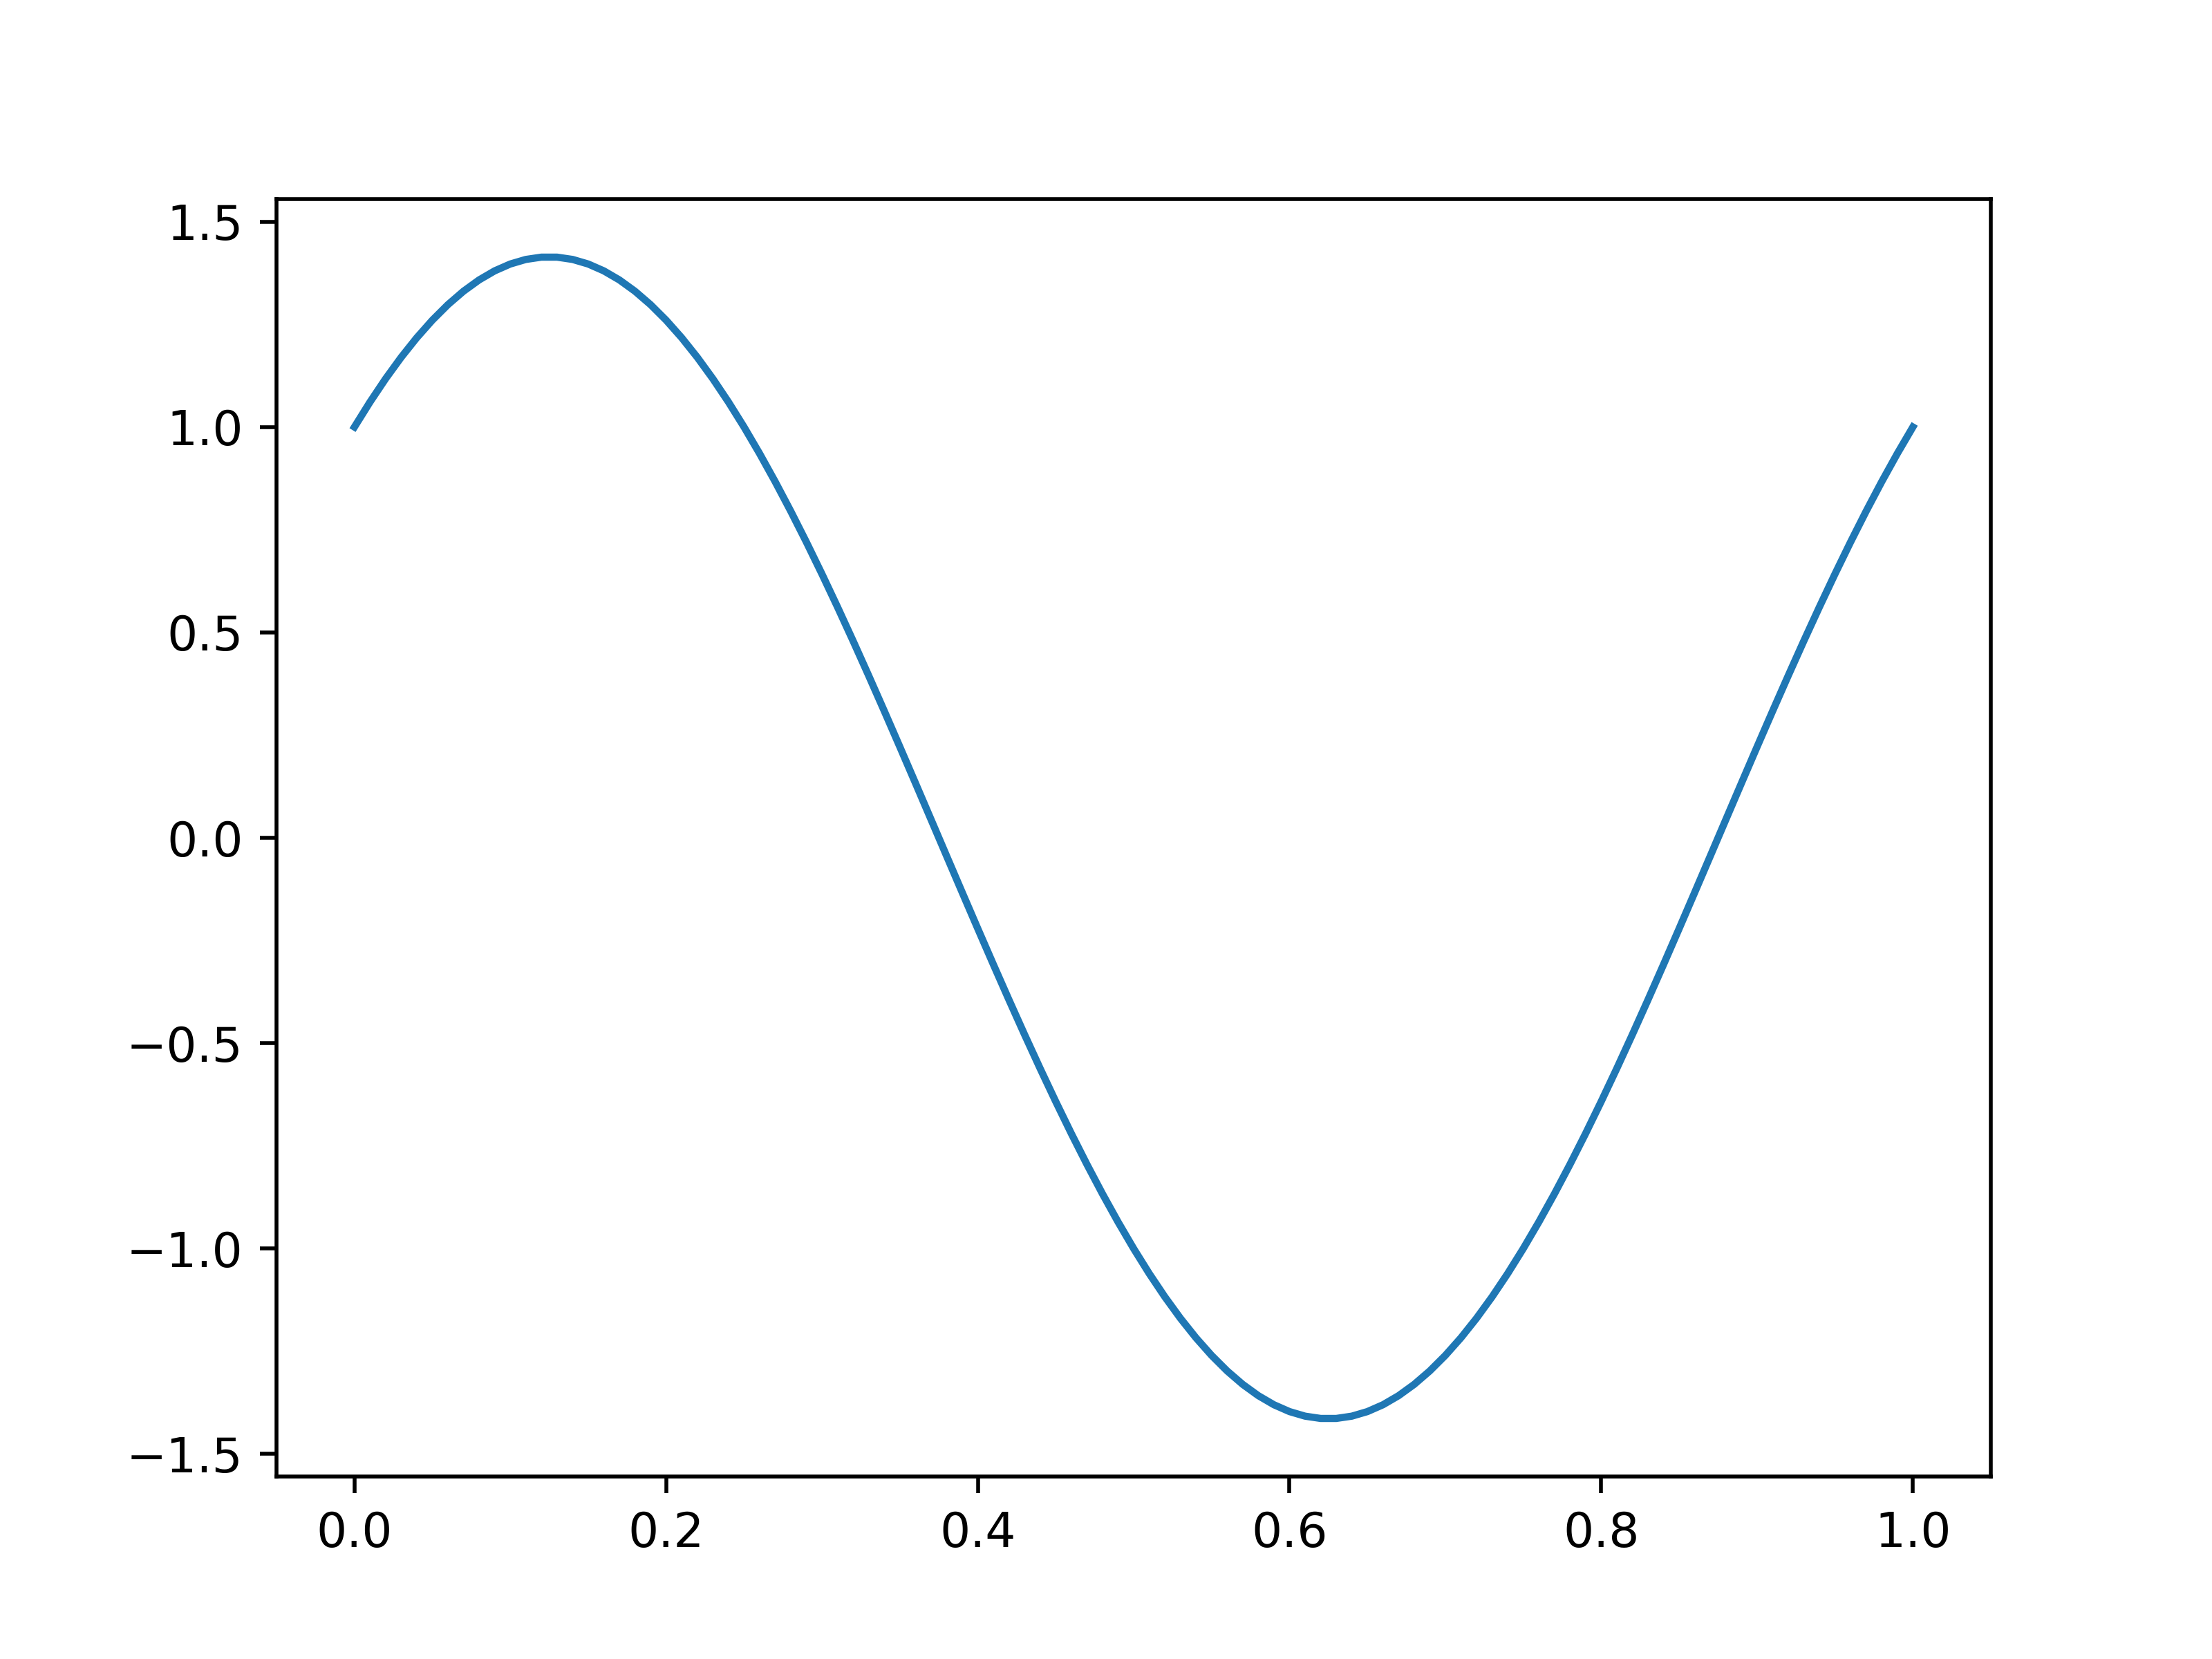
\includegraphics[width=\textwidth]{a1img1.png}
\caption{Lissajous figures for integer frequency ratios. Across rows and then down columns, the x:y frequency ratios are 1:1, 1:2, 1:3, and 1:4 respectively. The ratio $\frac{f_y}{f_x}$ gives the number of peaks (or equivalently the number of troughs) on the graph for one oscillation in X (i.e. one "peak" on the right side and one "peak" on the left). The figures shown here correspond to the parameters $A_x = A_y = 1, \Phi = \frac{\pi}{4}, \Delta t = 0.001,\text{ and }N = 1000.$}
\end{figure}
\begin{figure}[H]
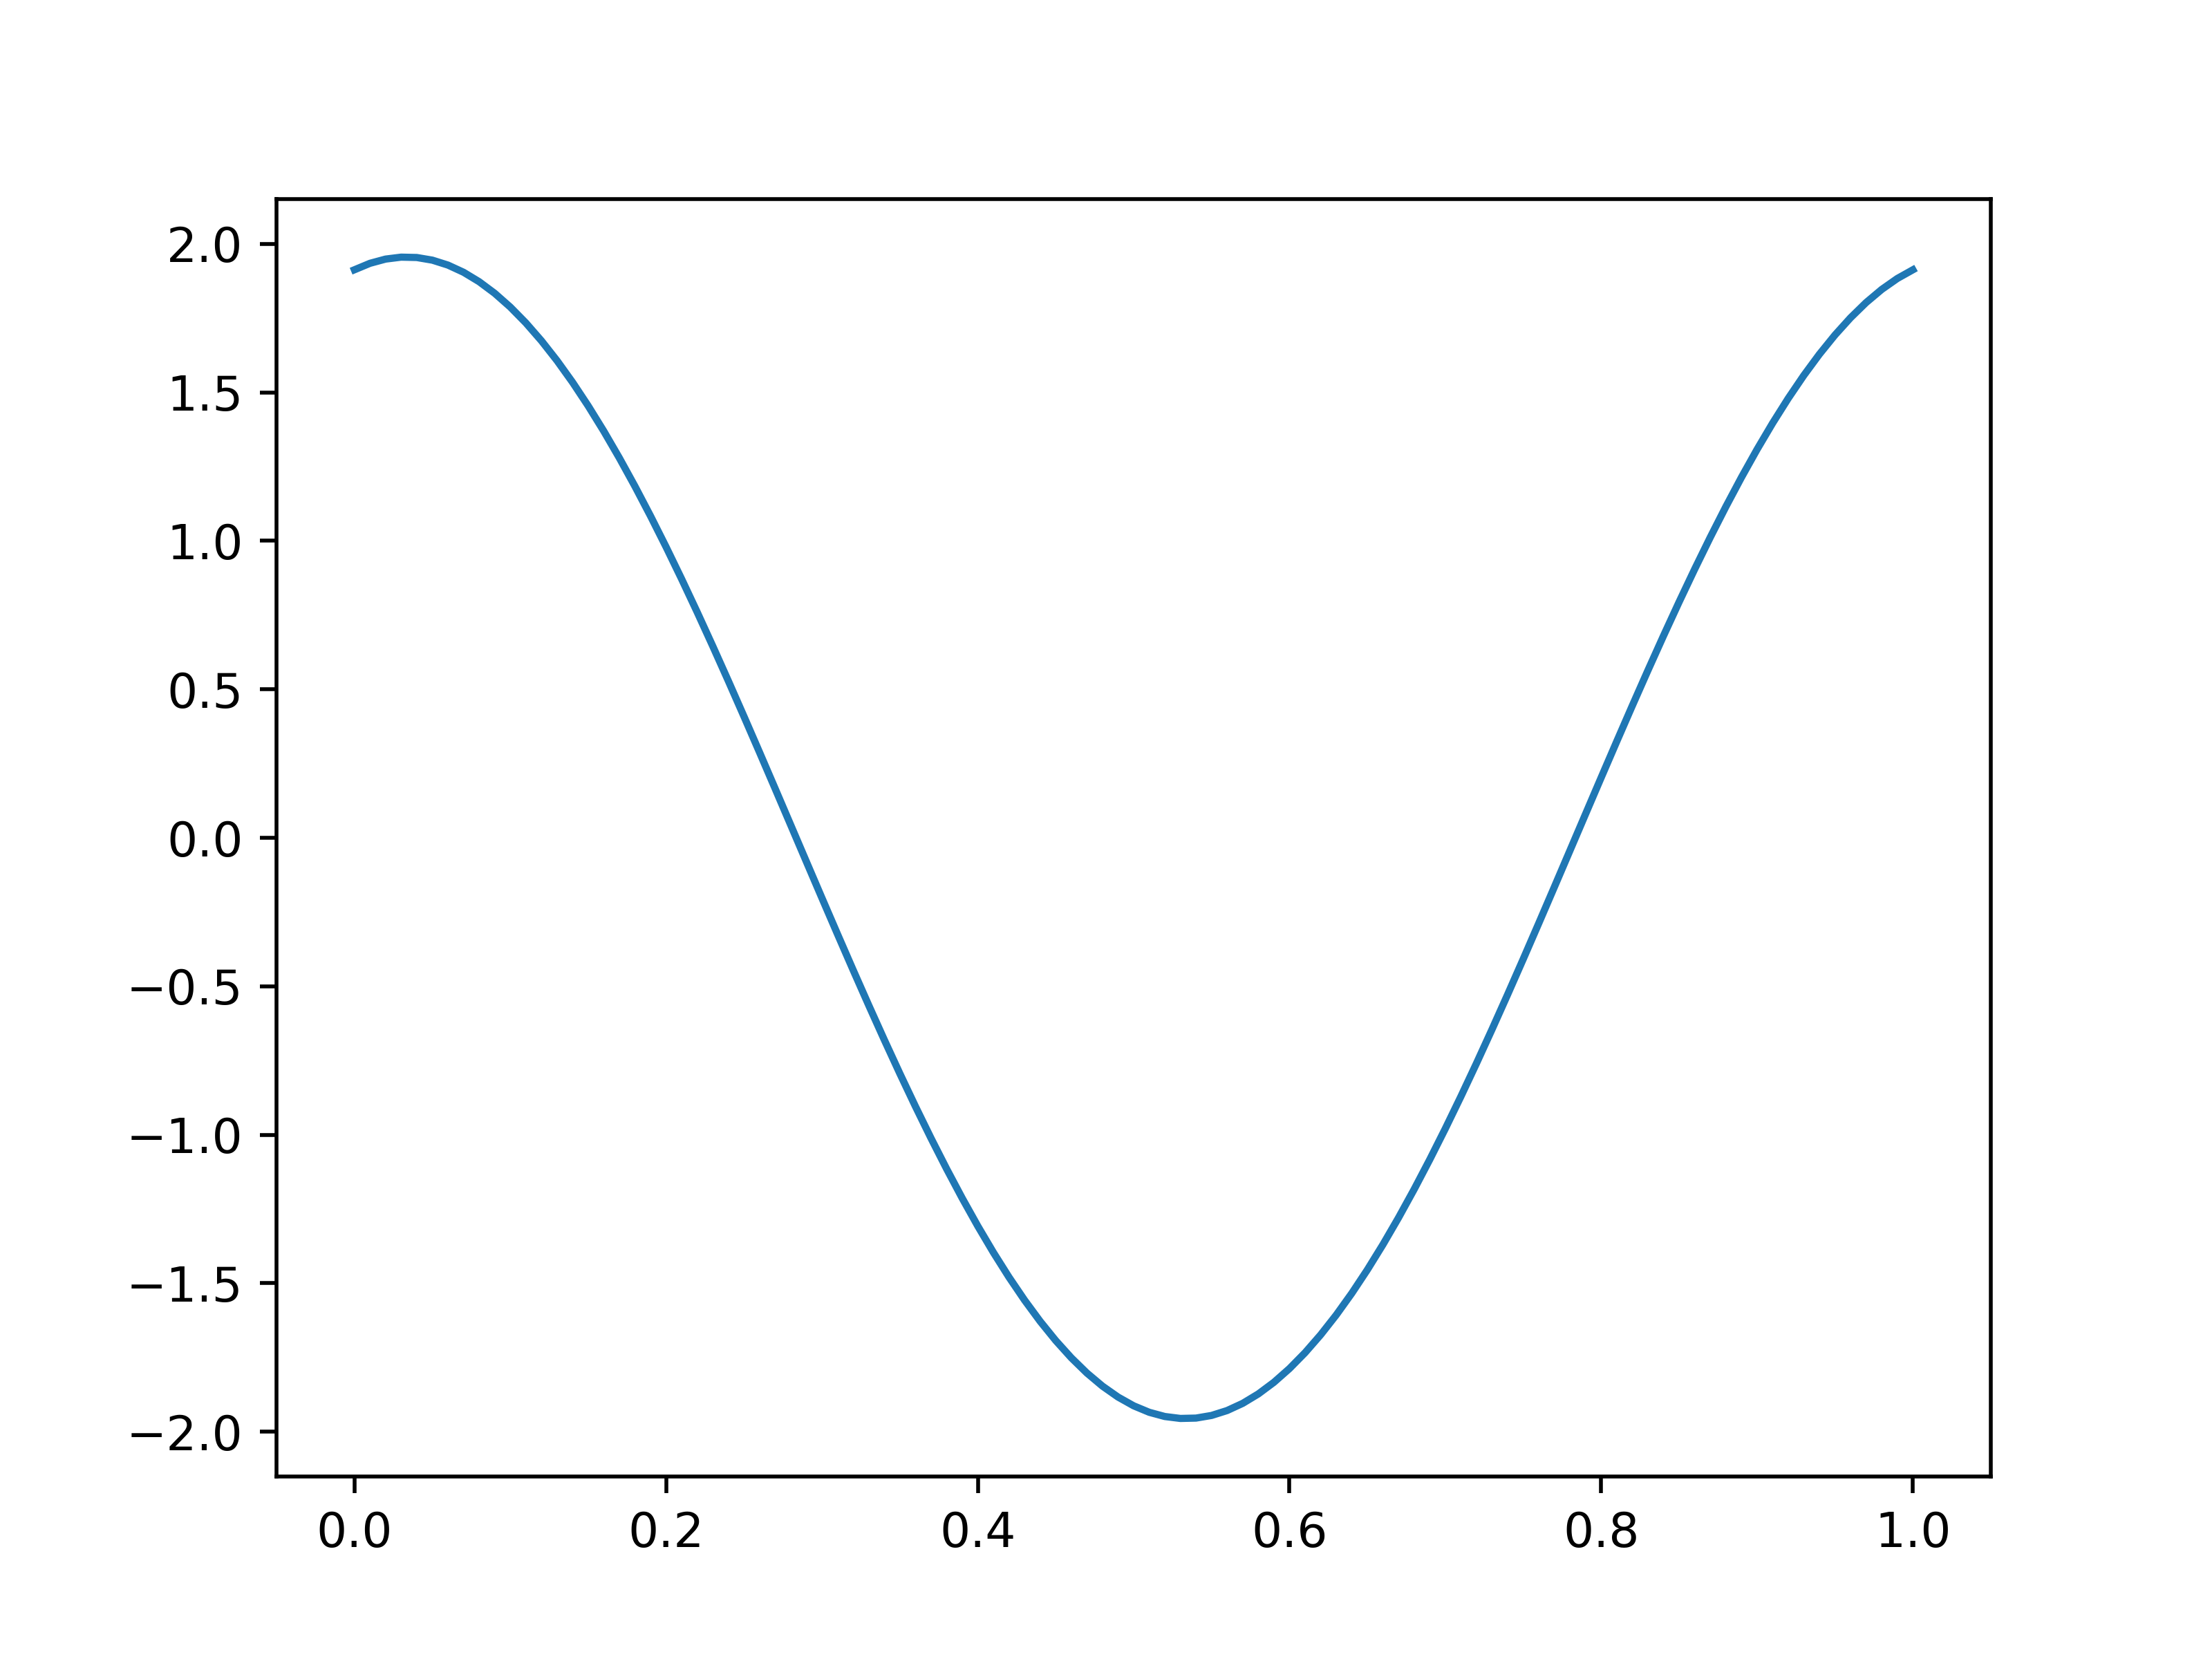
\includegraphics[width=\textwidth]{a1img2.png}
\caption{Lissajous figures for integer frequency ratios. Across rows and then down columns, the x:y frequency ratios are 1:1, 1:2, 1:3, and 1:4 respectively. The ratio $\frac{f_y}{f_x}$ gives the number of peaks (or equivalently the number of troughs) on the graph for one oscillation in X (i.e. one "peak" on the right side and one "peak" on the left). The figures shown here correspond to the parameters $A_x = A_y = 1, \Phi = \frac{\pi}{4}, \Delta t = 0.001,\text{ and }N = 1000.$}
\end{figure}
\begin{figure}[H]
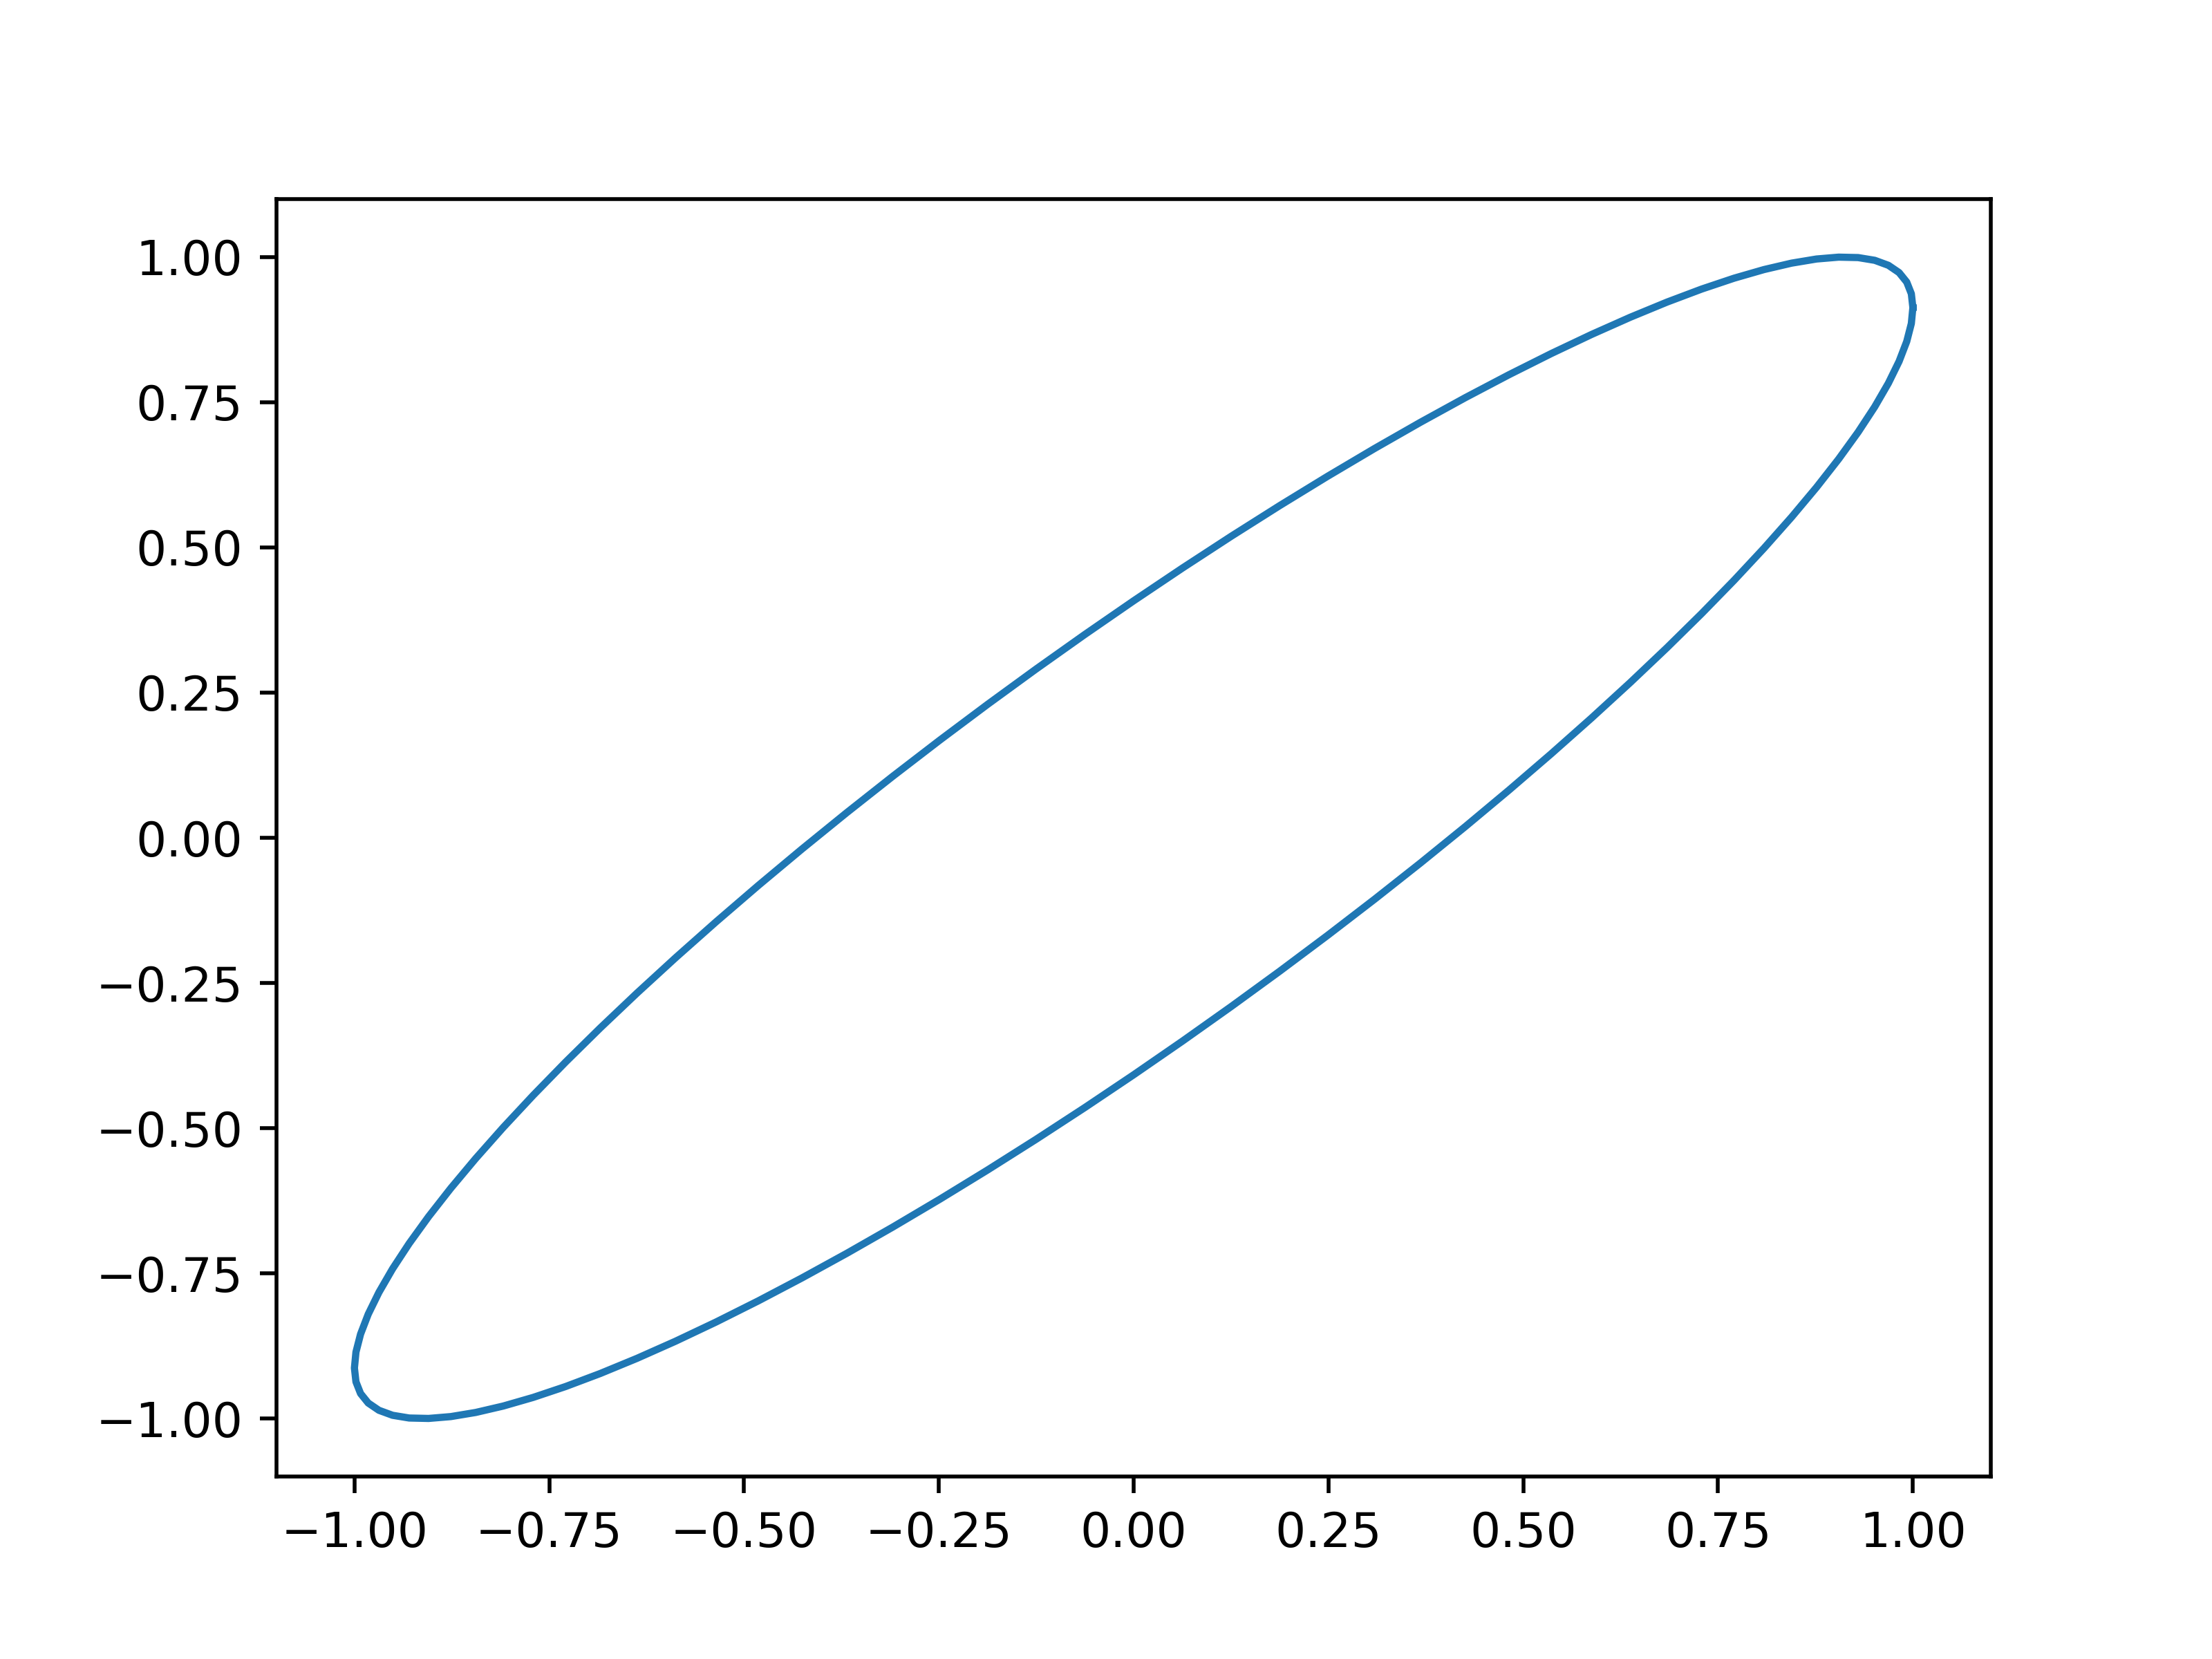
\includegraphics[width=\textwidth]{a1img3.png}
\caption{Lissajous figures for integer frequency ratios. Across rows and then down columns, the x:y frequency ratios are 1:1, 1:2, 1:3, and 1:4 respectively. The ratio $\frac{f_y}{f_x}$ gives the number of peaks (or equivalently the number of troughs) on the graph for one oscillation in X (i.e. one "peak" on the right side and one "peak" on the left). The figures shown here correspond to the parameters $A_x = A_y = 1, \Phi = \frac{\pi}{4}, \Delta t = 0.001,\text{ and }N = 1000.$}
\end{figure}
\end{document}